%%%%%%%%%%%%%%%%%%%%%%%% ExtendedAbstract.tex %%%%%%%%%%%%%%%%%%%%%%%%
%                                                                    %
%  Template for the 10-page extended abstract to be submitted for    %
%  the MSc degree conferral at Instituto Superior Tecnico.           %
%                                                                    %
%  Author:                                                           %
%                                                                    %
%       Andre C. Marta                                               %
%       Area Cientifica de Mecanica Aplicada e Aeroespacial          %
%       Departamento de Engenharia Mecanica                          %
%       Instituto Superior Tecnico                                   %
%       Av. Rovisco Pais                                             %
%       1049-001 Lisboa                                              %
%       Portugal                                                     %
%       Tel: +351 21 841 9466                                        %
%                        3466 (extension)                            %
%       Email: andre.marta@ist.utl.pt                                %
%                                                                    %
%  Created:       Dec  2, 2011                                       %
%  Last Modified: Dec 27, 2011                                       %
%%%%%%%%%%%%%%%%%%%%%%%%%%%%%%%%%%%%%%%%%%%%%%%%%%%%%%%%%%%%%%%%%%%%%%
% This document uses the LaTeX class file "article.cls"              %
%%%%%%%%%%%%%%%%%%%%%%%%%%%%%%%%%%%%%%%%%%%%%%%%%%%%%%%%%%%%%%%%%%%%%%
\documentclass[10pt,a4paper,twocolumn]{article}

%%%%%%%%%%%%%%%%%%%%%%%%%%%%%%%%%%%%%%%%%%%%%%%%%%%%%%%%%%%%%%%%%%%%%%
% Document preamble
%%%%%%%%%%%%%%%%%%%%%%%%%%%%%%%%%%%%%%%%%%%%%%%%%%%%%%%%%%%%%%%%%%%%%%

%% Builds upon the graphics  package, providing a key-value interface
%% for optional arguments to the \includegraphics command that go far
%% beyone what the graphics package offers.
%% http://www.ctan.org/tex-archive/help/Catalogue/entries/graphicx.html
%% if you use PostScript figures in your article
%% use the graphics package for simple commands
%% \usepackage{graphics}
%% or use the graphicx package for more complicated commands
%% \usepackage{graphicx}
%% or use the epsfig package if you prefer to use the old commands
%% \usepackage{epsfig}
\usepackage{graphicx} % Enhanced LaTeX Graphics

% Multiple figures
\usepackage{subfigure} % subcaptions for subfigures
\usepackage{subfigmat} % matrices of similar subfigures

% Declaring new column types
% 'dcolumn' package defines D to be a column specifier with
% three arguments: D{<sep.tex>}{<sep.dvi>}{<decimal places>}
%                  D{<sep.tex>}{<sep.dvi>}{<left digit places>.<right digit places>}
\usepackage{dcolumn}           % decimal-aligned tabular math columns
% d takes a single argument specifying the number of decimal places, e.g., d{2}
% or the number of digits to the left and right of the seperator, e.g., d{3.2}
\newcolumntype{.}   {D{.}{.}{-1}} % column alignedd on the point separator '.'
\newcolumntype{d}[1]{D{.}{.}{#1}} % column centered on the point separator '.'
\newcolumntype{e}   {D{E}{E}{-1}} % column centered on the exponent 'E'
\newcolumntype{E}[1]{D{E}{E}{#1}} % column centered on the exponent 'E'

%% American Mathematical Society (AMS) plain Tex macros
%%
%% The amsmath package is the principal package in the AMS-LaTeX distribution
%% http://www.ctan.org/tex-archive/help/Catalogue/entries/amsmath.html
\usepackage{amsmath}
%%
%% The amsfonts package provides extended TeX fonts
%% http://www.ctan.org/tex-archive/help/Catalogue/entries/amsfonts.html
\usepackage{amsfonts}
%% The amssymb package provides various useful mathematical symbols
\usepackage{amssymb}
%%
%% The amsthm package provides extended theorem environments
%% http://www.ctan.org/tex-archive/help/Catalogue/entries/amsthm.html
\usepackage{amsthm}

%% Improves the interface for defining floating objects such as figures and tables.
%% The package also provides the H float modifier option of the obsolete here package.
%% http://www.ctan.org/tex-archive/help/Catalogue/entries/float.html
\usepackage{float}

%% Control sectional headers. 
%% http://www.ctan.org/tex-archive/help/Catalogue/entries/sectsty.html
\usepackage{sectsty}
%%
%% Redefine the font size of the 'section' and 'subsection' headings
\newcommand{\myFontSize}{\fontsize{10}{0}\selectfont}
\sectionfont{\myFontSize}       % 10pt, Bold face (default)
\subsectionfont{\rm\myFontSize} % 10pt, Plain face

%% Select alternative section titles.
%% http://www.ctan.org/tex-archive/help/Catalogue/entries/titlesec.html
\usepackage{titlesec}
%%
%% Left indent, before and after spacing
%% (The starred version kills the indentation of the paragraph following the title)
\titlespacing*{\section}{0pt}{10pt}{0pt}
\titlespacing*{\subsection}{0pt}{10pt}{0pt}

%% Section numbers with trailing dots. 
%% http://www.ctan.org/tex-archive/help/Catalogue/entries/secdot.html
\usepackage{secdot}
%%
%% Also put a dot after the subsection number
\sectiondot{subsection}
%% Set a space between dot and heading text
\sectionpunct{section}{. }    % By default, \sectiondot places a \quad
\sectionpunct{subsection}{. } % after the number

% These are exact settings for a A4 page with top margin of
% 25 mm, bottom margin of 30 mm, left and right margins of 25 mm,
% printable area 242 X 160 mm.

\setlength{\topmargin}{-10.4mm}
\setlength{\headheight}{0.0mm}
\setlength{\headsep}{10.0mm}
\setlength{\textwidth}{160mm}
\setlength{\textheight}{242mm}
\setlength{\oddsidemargin}{0mm}
\setlength{\evensidemargin}{0mm}
\setlength{\marginparwidth}{0mm}
\setlength{\marginparsep}{0mm}

% New command to refer to equations as Eq.(1),Eq.(2),...
\newcommand{\eqnref}[1]{Eq.(\ref{#1})}

%%%%%%%%%%%%%%%%%%%%%%%%%%%%%%%%%%%%%%%%%%%%%%%%%%%%%%%%%%%%%%%%%%%%%%%%%%%%%%%%%%%%%%%%
% Title, authors and addresses

\title{Title of the MsC Thesis}
\date{December 2011}
\author{Name of author \\ author.name@ist.utl.pt \\ \\ Instituto Superior T\'{e}cnico, Lisboa, Portugal}

%%%%%%%%%%%%%%%%%%%%%%%%%%%%%%%%%%%%%%%%%%%%%%%%%%%%%%%%%%%%%%%%%%%%%%%%%%%%%%%%%%%%%%%%
\begin{document}

% Begin one column section for title and abstract
%
% http://www.faqs.org/faqs/de-tex-faq/part5/
\twocolumn[
\begin{@twocolumnfalse}
\maketitle

%%%%%%%%%%%%%%%%%%%%%%%%%%%%%%%%%%%%%%%%%%%%%%%%%%%%%%%%%%%%%%%%%%%%%%
% ABSTRACT & KEYWORDS
%%%%%%%%%%%%%%%%%%%%%%%%%%%%%%%%%%%%%%%%%%%%%%%%%%%%%%%%%%%%%%%%%%%%%%
%%%%%%%%%%%%%%%%%%%%%%%%%%%%%%%%%%%%%%%%%%%%%%%%%%%%%%%%%%%%%%%%%%%%%%
%     File: ExtendedAbstract_abstr.tex                               %
%     Tex Master: ExtendedAbstract.tex                               %
%                                                                    %
%     Author: Andre Calado Marta                                     %
%     Last modified : 2 Dez 2011                                     %
%%%%%%%%%%%%%%%%%%%%%%%%%%%%%%%%%%%%%%%%%%%%%%%%%%%%%%%%%%%%%%%%%%%%%%
% The abstract of should have less than 500 words.
% The keywords should be typed here (three to five keywords).
%%%%%%%%%%%%%%%%%%%%%%%%%%%%%%%%%%%%%%%%%%%%%%%%%%%%%%%%%%%%%%%%%%%%%%

%%
%% Abstract
%%
\begin{abstract}

Place abstract here.
%
No paragraph breaks.
\\
%%
%% Keywords (max 5)
%%
\noindent{{\bf Keywords:}} Keyword1, Keyword2, Keyword3, Keyword4, Keyword5 \\

\end{abstract}



% End one column section (begin default two columns)
\end{@twocolumnfalse}
]
%%%%%%%%%%%%%%%%%%%%%%%%%%%%%%%%%%%%%%%%%%%%%%%%%%%%%%%%%%%%%%%%%%%%%%
% INTRODUCTION
%%%%%%%%%%%%%%%%%%%%%%%%%%%%%%%%%%%%%%%%%%%%%%%%%%%%%%%%%%%%%%%%%%%%%%
%%%%%%%%%%%%%%%%%%%%%%%%%%%%%%%%%%%%%%%%%%%%%%%%%%%%%%%%%%%%%%%%%%%%%%
%     File: ExtendedAbstract_intro.tex                               %
%     Tex Master: ExtendedAbstract.tex                               %
%                                                                    %
%     Author: Andre Calado Marta                                     %
%     Last modified : 27 Dez 2011                                    %
%%%%%%%%%%%%%%%%%%%%%%%%%%%%%%%%%%%%%%%%%%%%%%%%%%%%%%%%%%%%%%%%%%%%%%
% State the objectives of the work and provide an adequate background,
% avoiding a detailed literature survey or a summary of the results.
%%%%%%%%%%%%%%%%%%%%%%%%%%%%%%%%%%%%%%%%%%%%%%%%%%%%%%%%%%%%%%%%%%%%%%

\section{Introduction}
\label{sec:intro}

Motivation and state-of-the-art...

Include relevant references~\cite{nocedal:opt}.



%%%%%%%%%%%%%%%%%%%%%%%%%%%%%%%%%%%%%%%%%%%%%%%%%%%%%%%%%%%%%%%%%%%%%%
% BACKGROUND
%%%%%%%%%%%%%%%%%%%%%%%%%%%%%%%%%%%%%%%%%%%%%%%%%%%%%%%%%%%%%%%%%%%%%%
%%%%%%%%%%%%%%%%%%%%%%%%%%%%%%%%%%%%%%%%%%%%%%%%%%%%%%%%%%%%%%%%%%%%%%
%     File: ExtendedAbstract_backg.tex                               %
%     Tex Master: ExtendedAbstract.tex                               %
%                                                                    %
%     Author: Andre Calado Marta                                     %
%     Last modified : 27 Dez 2011                                    %
%%%%%%%%%%%%%%%%%%%%%%%%%%%%%%%%%%%%%%%%%%%%%%%%%%%%%%%%%%%%%%%%%%%%%%
% A Theory section should extend, not repeat, the background to the
% article already dealt with in the Introduction and lay the
% foundation for further work.
%%%%%%%%%%%%%%%%%%%%%%%%%%%%%%%%%%%%%%%%%%%%%%%%%%%%%%%%%%%%%%%%%%%%%%

\section{Background}
\label{sec:backg}

Place text here...


%%%%%%%%%%%%%%%%%%%%%%%%%%%%%%%%%%%%%%%%%%%%%%%%%%%%%%%%%%%%%%%%%%%%%%
\subsection{Sub-section...}

A generic CFD design problem can be formally described as
%
\begin{eqnarray}
  {\rm Minimize}   && Y({\bf \alpha},{\bf q}({\bf \alpha}))            \nonumber           \\
  {\rm w.r.t.}     && {\bf \alpha} \,,                                 \label{eq:minimize} \\
  {\rm subject~to} && {\cal R}({\bf \alpha},{\bf q}({\bf \alpha})) = 0 \nonumber           \\
                   &&       C ({\bf \alpha},{\bf q}({\bf \alpha})) = 0 \,, \nonumber
\end{eqnarray}
%
where $Y$ is the cost function, ${\bf \alpha}$ is the vector of design variables and ${\bf q}$ is the flow solution, which is typically of function of the design variables, and $C = 0$ represents additional constraints that may or may not involve the flow solution.
%
The flow governing equations expressed in the form ${\cal R} = 0$ also appear as a constraint, as the solution ${\bf q}$ must always obey the flow physics.


%%%%%%%%%%%%%%%%%%%%%%%%%%%%%%%%%%%%%%%%%%%%%%%%%%%%%%%%%%%%%%%%%%%%%%
\subsection{Sub-section...}

More text...


%%%%%%%%%%%%%%%%%%%%%%%%%%%%%%%%%%%%%%%%%%%%%%%%%%%%%%%%%%%%%%%%%%%%%%
% IMPLEMENTATION
%%%%%%%%%%%%%%%%%%%%%%%%%%%%%%%%%%%%%%%%%%%%%%%%%%%%%%%%%%%%%%%%%%%%%%
%%%%%%%%%%%%%%%%%%%%%%%%%%%%%%%%%%%%%%%%%%%%%%%%%%%%%%%%%%%%%%%%%%%%%%
%     File: ExtendedAbstract_imple.tex                               %
%     Tex Master: ExtendedAbstract.tex                               %
%                                                                    %
%     Author: Andre Calado Marta                                     %
%     Last modified : 27 Dez 2011                                    %
%%%%%%%%%%%%%%%%%%%%%%%%%%%%%%%%%%%%%%%%%%%%%%%%%%%%%%%%%%%%%%%%%%%%%%
% A Calculation section represents a practical development
% from a theoretical basis.
%%%%%%%%%%%%%%%%%%%%%%%%%%%%%%%%%%%%%%%%%%%%%%%%%%%%%%%%%%%%%%%%%%%%%%

\section{Implementation}
\label{sec:imple}

Place text here...


%%%%%%%%%%%%%%%%%%%%%%%%%%%%%%%%%%%%%%%%%%%%%%%%%%%%%%%%%%%%%%%%%%%%%%
\subsection{Sub-section...}

More text...


%%%%%%%%%%%%%%%%%%%%%%%%%%%%%%%%%%%%%%%%%%%%%%%%%%%%%%%%%%%%%%%%%%%%%%
\subsection{Sub-section...}

More text...



%%%%%%%%%%%%%%%%%%%%%%%%%%%%%%%%%%%%%%%%%%%%%%%%%%%%%%%%%%%%%%%%%%%%%%
% RESULTS
%%%%%%%%%%%%%%%%%%%%%%%%%%%%%%%%%%%%%%%%%%%%%%%%%%%%%%%%%%%%%%%%%%%%%%
%%%%%%%%%%%%%%%%%%%%%%%%%%%%%%%%%%%%%%%%%%%%%%%%%%%%%%%%%%%%%%%%%%%%%%
%     File: ExtendedAbstract_resul.tex                               %
%     Tex Master: ExtendedAbstract.tex                               %
%                                                                    %
%     Author: Andre Calado Marta                                     %
%     Last modified : 27 Dez 2011                                    %
%%%%%%%%%%%%%%%%%%%%%%%%%%%%%%%%%%%%%%%%%%%%%%%%%%%%%%%%%%%%%%%%%%%%%%
% Results
% Results should be clear and concise.
% Discussion
% This should explore the significance of the results of the work, not
% repeat them. A combined Results and Discussion section is often
% appropriate. Avoid extensive citations and discussion of published
% literature.
%%%%%%%%%%%%%%%%%%%%%%%%%%%%%%%%%%%%%%%%%%%%%%%%%%%%%%%%%%%%%%%%%%%%%%

\section{Results}
\label{sec:resul}

Place text here...


%%%%%%%%%%%%%%%%%%%%%%%%%%%%%%%%%%%%%%%%%%%%%%%%%%%%%%%%%%%%%%%%%%%%%%
\subsection{Sub-section...}

More text...

Figure~\ref{fig:blade_flow_pressure} shows the contour of pressure on the hub and blade surface planes corresponding to the baseline blade geometry.

\begin{figure}[H]
  \centering
  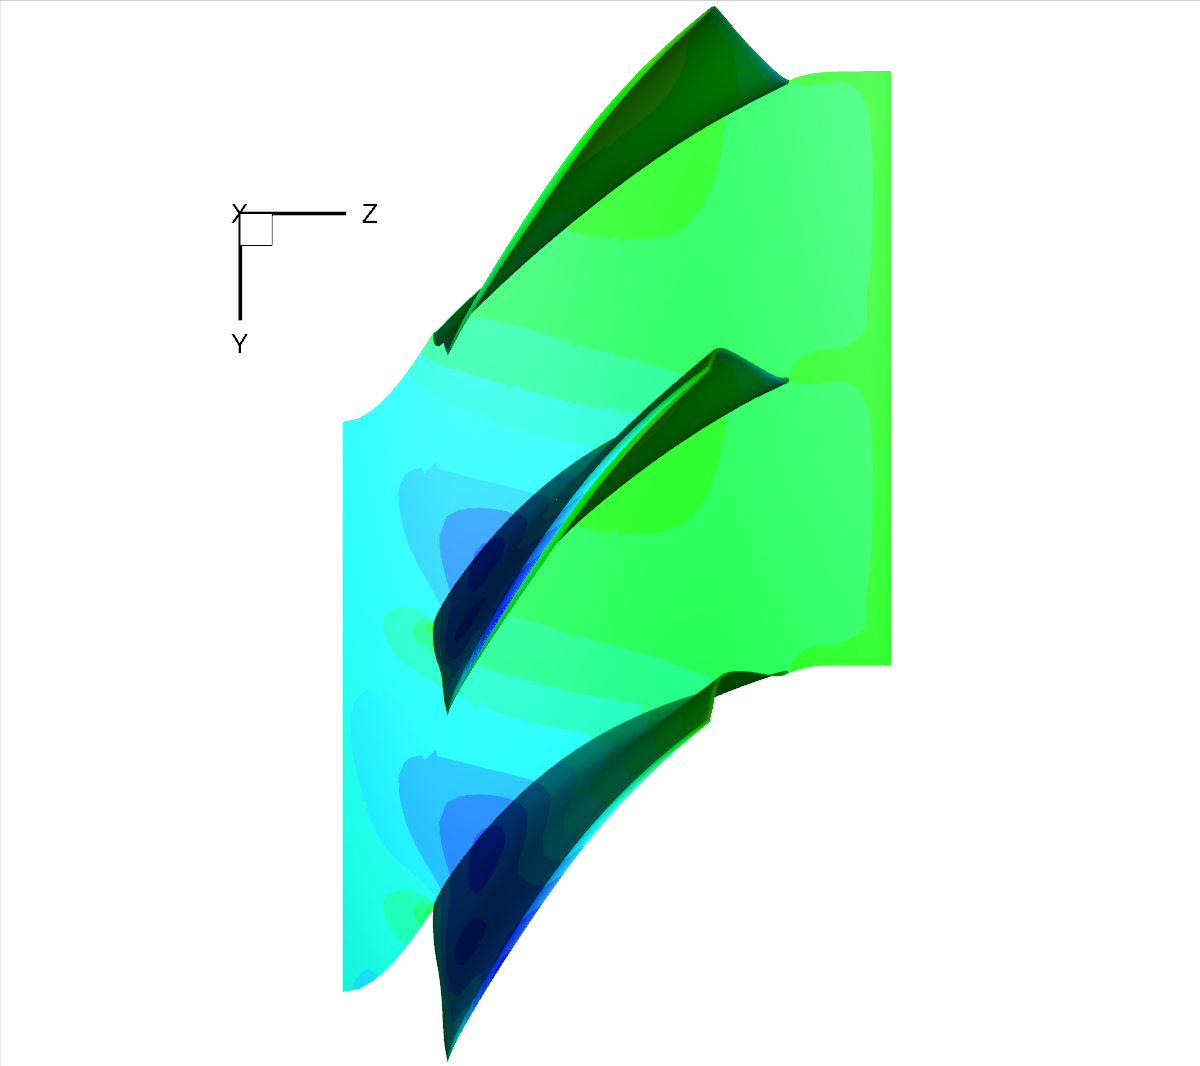
\includegraphics[width=5cm]{images/master_flow.png}
  \caption{Pressure distribution.}
  \label{fig:blade_flow_pressure}
\end{figure}

As seen in Fig.\ref{fig:blade_flow_pressure}...


%%%%%%%%%%%%%%%%%%%%%%%%%%%%%%%%%%%%%%%%%%%%%%%%%%%%%%%%%%%%%%%%%%%%%%
\subsection{Sub-section...}

More text...

Table~\ref{table:simple} summarizes...

\begin{table}[!h]
  \begin{center}
    \begin{tabular}{lccc}
      Model           & $C_L$ & $C_D$ & $C_{M y}$ \\
      \hline
      Euler           & 0.083 & 0.021 & -0.110    \\
      Navier--Stokes  & 0.078 & 0.023 & -0.101    \\
      \hline
    \end{tabular}
  \end{center}
  \caption[Table caption shown in TOC]{Table caption}
  \label{table:simple}
\end{table}

As seen in Tab.\ref{table:simple}...



%%%%%%%%%%%%%%%%%%%%%%%%%%%%%%%%%%%%%%%%%%%%%%%%%%%%%%%%%%%%%%%%%%%%%%
% CONCLUSIONS
%%%%%%%%%%%%%%%%%%%%%%%%%%%%%%%%%%%%%%%%%%%%%%%%%%%%%%%%%%%%%%%%%%%%%%
%%%%%%%%%%%%%%%%%%%%%%%%%%%%%%%%%%%%%%%%%%%%%%%%%%%%%%%%%%%%%%%%%%%%%%
%     File: ExtendedAbstract_concl.tex                               %
%     Tex Master: ExtendedAbstract.tex                               %
%                                                                    %
%     Author: Andre Calado Marta                                     %
%     Last modified : 27 Dez 2011                                    %
%%%%%%%%%%%%%%%%%%%%%%%%%%%%%%%%%%%%%%%%%%%%%%%%%%%%%%%%%%%%%%%%%%%%%%
% The main conclusions of the study presented in short form.
%%%%%%%%%%%%%%%%%%%%%%%%%%%%%%%%%%%%%%%%%%%%%%%%%%%%%%%%%%%%%%%%%%%%%%

\section{Conclusions}
\label{sec:concl}

Conclusions, future work and some final remarks...



%%%%%%%%%%%%%%%%%%%%%%%%%%%%%%%%%%%%%%%%%%%%%%%%%%%%%%%%%%%%%%%%%%%%%%
% ACKNOWLEDGMENTS
%%%%%%%%%%%%%%%%%%%%%%%%%%%%%%%%%%%%%%%%%%%%%%%%%%%%%%%%%%%%%%%%%%%%%%
%%%%%%%%%%%%%%%%%%%%%%%%%%%%%%%%%%%%%%%%%%%%%%%%%%%%%%%%%%%%%%%%%%%%%%
%     File: ExtendedAbstract_ackno.tex                               %
%     Tex Master: ExtendedAbstract.tex                               %
%                                                                    %
%     Author: Andre Calado Marta                                     %
%     Last modified : 27 Dez 2011                                    %
%%%%%%%%%%%%%%%%%%%%%%%%%%%%%%%%%%%%%%%%%%%%%%%%%%%%%%%%%%%%%%%%%%%%%%
% Acknowledge persons and institutions that supported this work.
%%%%%%%%%%%%%%%%%%%%%%%%%%%%%%%%%%%%%%%%%%%%%%%%%%%%%%%%%%%%%%%%%%%%%%

\section*{Acknowledgements}

The author would like to thank ...



%%%%%%%%%%%%%%%%%%%%%%%%%%%%%%%%%%%%%%%%%%%%%%%%%%%%%%%%%%%%%%%%%%%%%%
% REFERENCES
%%%%%%%%%%%%%%%%%%%%%%%%%%%%%%%%%%%%%%%%%%%%%%%%%%%%%%%%%%%%%%%%%%%%%%

% Produces the bibliography section when processed by BibTeX
%
% Bibliography style
% > entries ordered alphabetically
%\bibliographystyle{plain}
% > unsorted with entries appearing in the order in which the citations appear.
%\bibliographystyle{unsrt}
% > entries ordered alphabetically, with first names and names of journals and months abbreviated
\bibliographystyle{abbrv}
% > entries ordered alphabetically, with reference markers based on authors' initials and publication year
%\bibliographystyle{alpha}

% External bibliography database file in the BibTeX format (ExtendedAbstract_ref_db.bib)
\bibliography{ExtendedAbstract_ref_db}

%%%%%%%%%%%%%%%%%%%%%%%%%%%%%%%%%%%%%%%%%%%%%%%%%%%%%%%%%%%%%%%%%%%%%%
\end{document}
%%%%%%%%%%%%%%%%%%%%%%%%%%%%%%%%%%%%%%%%%%%%%%%%%%%%%%%%%%%%%%%%%%%%%%

